\documentclass[hyperref=colorlinks]{beamer}
\mode<presentation>
\usetheme{iclpt}
\setbeamertemplate{navigation symbols}{}
\setbeamertemplate{headline}{
\begin{beamercolorbox}[leftskip=.2cm,rightskip=.2cm,topskip=.2cm,ht=1.1cm,dp=0.1cm,wd=\textwidth]{institute in head/foot}
  
\includegraphics[height=1cm]{icl.pdf}
  \hfill
  
\includegraphics[height=1cm]{../Pics/CMS-Color.pdf}
\end{beamercolorbox}
}
\setbeamertemplate{footline}{
\begin{beamercolorbox}[ht=.55cm,dp=0.4cm,wd=\textwidth,leftskip=.3cm]{author in head/foot}%
  \begin{minipage}[c]{5cm}%
    \usebeamerfont{author in head/foot}
    \insertshortauthor 
    \insertshorttitle
    \end{minipage}\hfill%
  \insertframenumber{} / \pageref{lastframe}
  \hfill
  \begin{minipage}{6cm}
    \hfill
  \end{minipage}
\end{beamercolorbox}%
}

\usepackage{color}
\usepackage{tabularx,colortbl}
\usepackage{graphicx}
\usepackage{pdfpages}
\usepackage{feynmp}
\DeclareGraphicsRule{*}{mps}{*}{}

\title{\vspace{-0.2cm} Framework Progress Update}
%\subtitle{Paper - HIG-13-030, PASs: HIG-13-013, HIG-13-018, HIG-13-028 \vspace{-0.7cm}}
\author[P. Dunne]{\underline{P. Dunne} }%\\ on behalf of the H$\rightarrow$invisible analysis groups} % A.M. Magnan and A. Nikitenko Joao Pela with \\ R. Aggleton, J. Brooke: Bristol \\ C.Asawangtrakuldee, Q.Li: Peking \\ P. Srimanobhas: Chulalongkorn \\ S. Kumar, K. Mazumdar: Mumbai}
\titlegraphic{
  \vspace{-0.7cm}
  %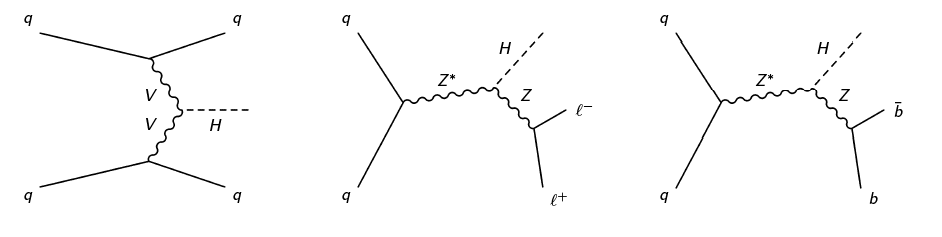
\includegraphics[width=\textwidth]{TalkPics/invcomb021213/feyndiags}
%% \begin{fmfgraph*}(100,70)
%%         \fmfleft{i1,i2}
%%         \fmfright{o1,o2,o3}
%%         \fmf{fermion}{i1,v1,o1}
%%         \fmf{fermion}{i2,v2,o3}
%%         \fmf{phantom,tension=4/5}{v1,v2}
%%         \fmffreeze
%%         \fmf{photon,label=$W,,Z$}{v1,v3}
%%         \fmf{photon,label=$W,,Z$}{v2,v3}
%%         \fmf{dashes}{v3,o2}
%%         \fmflabel{$q$}{i1}
%%         \fmflabel{$q$}{i2}
%%         \fmflabel{$q$}{o1}
%%         \fmflabel{$q$}{o3}
%%         \fmflabel{$H$}{o2}
%%       \end{fmfgraph*}
}
\date{}
\begin{document}
\begin{fmffile}{hig1330approvalfeynmandiags}

%TITLE PAGE
\section{Title}
\begin{frame}
  \titlepage
  
\end{frame}

%OUTLINE
\begin{frame}
  \frametitle{Overview}
  \begin{block}{}
    \scriptsize
    \begin{itemize}
    \item Synchronisation update
    \item Twiki with instructions can be found \href{https://twiki.cern.ch/twiki/bin/viewauth/CMS/VBFHinvisibleParkedData}{here}
    \end{itemize}
  \end{block}
\end{frame}

\begin{frame}
  \frametitle{General progress update}
  \begin{columns}
    \column{1.1\textwidth}
  \begin{block}{}
    \scriptsize
    \begin{itemize}
    \item Light trees for all samples are accessible through xrootd:
    \item[-] Also have a skim with Joao and AMs QCD pre-selection (323MB)
    \item Scripts to support running the framework on the Imperial and CERN batch systems have been fixed.
    \end{itemize}
  \end{block}
  \end{columns}
\end{frame}

\begin{frame}
  \frametitle{W mu/e nu background synch}
  \begin{columns}
    \column{.5\textwidth}
    \begin{block}{}
      \begin{itemize}
      \item Fully synched already
      \item Remain in synch with the minor changes made for the other backgrounds described below
      \end{itemize}
    \end{block}
    \column{.5\textwidth}
    \begin{block}{}
      \centering
    \begin{tabular}{|l|c|c|}
      \hline
      Number & Old FW & New FW \\
      \hline
      $W\rightarrow\mu\nu$ & 65.1 & 65.1 \\
      $W\rightarrow e\nu$ & 68.3 & 68.3 \\
      \hline
    \end{tabular}
    \end{block}
  \end{columns}
\end{frame}

\begin{frame}
  \frametitle{Z background synch}
  \begin{columns}
    \column{.5\textwidth}
    \begin{block}{}
      \begin{itemize}
      \item Problem found with $m_{\mu\mu gen}$ variable
      \item[-] Fixed and now numbers agree
      \end{itemize}
    \end{block}
    \column{.5\textwidth}
    \begin{block}{}
      \centering
      \scriptsize
    \begin{tabular}{|l|c|c|}
      \hline
      Number & Old FW & New FW \\
      \hline
      NSMC EWK & 5.6 & 5.6 \\ 
      NSMC QCD & 26.0 & 26.0 \\
      NCMC EWK & 4.2 & 4.2 \\
      NCMC QCD & 20.2 & 20.2 \\
      NCData & 13 & 13 \\
      NCBkg & 0.15 & 0.15 \\
      \hline
      Result & 104.9 & 104.9 \\
      \hline
    \end{tabular}
    \end{block}
  \end{columns}
\end{frame}


\begin{frame}
  \frametitle{W taunu background synch}
  \begin{columns}
    \column{.5\textwidth}
    \begin{block}{}
      \begin{itemize}
      \item Existing W background module applied tight lepton ID weights to control region
      \item[-] $W\rightarrow\tau\nu$ background needs loose ID weights in control region
      \item Minor difference in control region selection identified
      \item[-] Old FW required ntaus$>=$1
      \item[-] New FW required ntaus==1
      \item Both issues fixed in new FW
      \end{itemize}
    \end{block}
    \column{.5\textwidth}
    \begin{block}{}
      \centering
    \begin{tabular}{|l|c|c|}
      \hline
      Number & Old FW & New FW \\
      \hline
      NSMC & 111.8 & 111.8 \\
      NCMC & 39.2 & 39.2 \\
      NCData & 30 & 30 \\
      NCBkg & 17.5 & 17.5 \\
      \hline
      Result & 35.7 & 35.7 \\
      \hline
    \end{tabular}
    \end{block}
  \end{columns}
\end{frame}

\begin{frame}
  \frametitle{QCD background synch}
  \begin{columns}
    \column{.5\textwidth}
    \begin{block}{}
      \begin{itemize}
      \item Old FW code revived
      \item[-] MC estimate of Z and W backgrounds is used instead of data driven
      \item New FW code written
      \item Agreed first time
      \end{itemize}
    \end{block}
    \column{.5\textwidth}
    \begin{block}{}
      \centering
      \scriptsize
    \begin{tabular}{|l|c|c|}
      \hline
      Number & Old FW & New FW \\
      \hline
      NAData & 5734 & 5734 \\
      NBData & 913 & 913 \\
      NCData & 810 & 810 \\
      NABkg & 190.2 & 190.2 \\
      NBBkg & 609.9 & 609.9 \\
      NCBkg & 66.5 & 66.5 \\
      \hline
      Result & 40.7 & 40.7 \\
      \hline
    \end{tabular}
    \end{block}
  \end{columns}
\end{frame}

\begin{frame}
  \frametitle{Conclusions}
  \label{lastframe}

  \begin{block}{}
    \scriptsize
    \begin{itemize}
    \item New framework now fully synched with old
    \item[-] Instructions to try it out can be found \href{https://twiki.cern.ch/twiki/bin/viewauth/CMS/VBFHinvisibleParkedData}{here}
    \item Light Ntuples are in DCache for old preselection and new preselection

    \end{itemize}
  \end{block}

\end{frame}

\begin{frame}
  \frametitle{Backup}
\end{frame}

\begin{frame}
  \frametitle{Paper BKG Estimates}
      \begin{block}{}
      \centering
      \scriptsize
    \begin{tabular}{|l|c|c|}
      \hline
      Background & Paper estimate & Rereco estimate \\
      \hline
      Zmumu & 99 & 105\\
      Wmunu & 67 & 65\\
      Wenu & 63 & 68\\
      Wtaunu & 53 & 36\\
      QCD & 31 & 41\\
      \hline
      Total & 313 & 315\\
      \hline
    \end{tabular}
    \end{block}
\end{frame}

\end{fmffile}
\end{document}
